% This text is proprietary.
% It's a part of presentation made by myself.
% It may not used commercial.
% The noncommercial use such as private and study is free
% Sep. 2005 
% Author: Sascha Frank 
% University Freiburg 
% www.informatik.uni-freiburg.de/~frank/


\documentclass[aspectratio=169]{beamer}
%\usetheme{Madrid}
\setbeamercovered{transparent=20}

%%% HANDOUT START
%  \documentclass[11pt,handout,aspectratio=169]{beamer}
%  \usepackage{pgfpages}
%  \pgfpagesuselayout{6 on 1}[a4paper]
%  \setbeamertemplate{footline}{% set footline options
%   $\qquad\qquad$\insertpagenumber   
%   }

 
%%% HANDOUT END

\usefonttheme{professionalfonts}
 
%\setbeamertemplate{page number in head/foot}[totalframenumber]
%\beamertemplatenavigationsymbolsempty

%\setbeamerfont{page number in head/foot}{size=\footnotesize}


%pdfnup --a4paper --keepinfo --nup 1x3 --frame true   --scale 0.92 --no-landscape --outfile handout.pdf slides.pdf


\setbeamercovered{transparent=10}


\usepackage{multirow}
% \usepackage{pgfpages}
% \mode<handout>{\setbeamercolor{background canvas}{bg=black!5}}
% \pgfpagesuselayout{4 on 1}[letterpaper,border shrink=2mm]

%\documentclass[handout]{beamer}
% \setbeamertemplate{bibliography entry title}{}
% \setbeamertemplate{bibliography entry location}{}
% \setbeamertemplate{bibliography entry note}{}
\setbeamertemplate{bibliography item}{\insertbiblabel}

\newcommand{\Prob}{{\rm I\hspace{-0.8mm}P}}

\newcommand{\p}[0]{\mathbf{p}}
\newcommand{\q}[0]{\mathbf{q}}

\newcommand{\e}[0]{\textbf{e}}
\newcommand{\PP}[0]{\mathbf{P}}
\newcommand{\II}[0]{\textbf{I}}
\newcommand{\Q}[0]{\mathbf{Q}}
\newcommand{\E}[0]{\mathbb{E}}
\newcommand{\X}[0]{\textbf{X}}
\newcommand{\Z}[0]{\textbf{Z}}
\newcommand{\s}[0]{\mathbf{s}}
\newcommand{\C}[0]{\textbf{C}}
\newcommand{\es}[0]{\mathbf{s}}
\newcommand{\trev}[0]{\overleftarrow}
\definecolor{mygray}{gray}{0.6}
\newcommand{\diag}{\mathbf{diag}}
\newcommand{\iii}[0]{\mathbf{i}}

%\dual to oznacznie dualnosci, oryginalnie *
%\newcommand{\dual}[0]{\circledast}
\newcommand{\dual}[0]{*}

%\monD to oznacznie tej drugiej monotonicznosci, czyli np. ^\monD-Mobius monotonicity
%\newcommand{\monD}[0]{\lozenge}
\newcommand{\monD}[0]{\downarrow}
\newcommand{\monU}[0]{\uparrow}

\usepackage{cancel} 

\usepackage{dsfont}
 
\newcommand{\indic}[0]{\mathds{1}}
\usepackage{pdfpages}
\usepackage{graphicx}
\usepackage{soul} 
\usepackage{tikz}
\usepackage[utf8]{inputenc}
\usepackage[T1]{fontenc}
\usetikzlibrary{arrows}
\usetikzlibrary{positioning}




\setbeamertemplate{theorems}[numbered]

% Add support for \subsubsectionpage
%\def\subsubsectionname{\translate{Subsubsection}}
%\def\insertsubsubsectionnumber{\arabic{subsubsection}}
% \setbeamertemplate{subsubsection page}
% {
%   \begin{centering}
%     {\usebeamerfont{subsubsection name}\usebeamercolor[fg]{subsubsection name}\subsubsectionname~\insertsubsubsectionnumber}
%     \vskip1em\par
% %     \begin{beamercolorbox}[sep=4pt,center]{d part title}
% %       \usebeamerfont{subsubsection title}\insertsubsubsection\par
% %     \end{beamercolorbox}
%   \end{centering}
% }
% \def\subsubsectionpage{\usebeamertemplate*{subsubsection page}}


\AtBeginSection{\frame{\sectionpage}}
\AtBeginSubsection{\frame{\subsectionpage}}
\AtBeginSubsubsection{\frame{\subsubsectionpage}}
 
\usepackage{tikz}

\usepackage{pgfplots}
\pgfplotsset{compat=1.11}
 

 % FROM BOOK:
 


\usepackage{algorithm}

\usepackage{algpseudocode}
\usepackage{caption}
\usepackage{comment}
\usepackage{booktabs}


 \usepackage[T1]{fontenc}
%\usepackage[utf8]{inputenc}
%\usepackage[polish]{babel}

\usepackage{tikz}
\usetikzlibrary{arrows}
\usetikzlibrary{arrows.meta}
\usetikzlibrary{patterns}
%\usetikzlibrary{decorations.pathreplacing,calligraphy}
\usetikzlibrary{decorations.text}
\usetikzlibrary{decorations.markings}
\usetikzlibrary{decorations.pathreplacing}
\usetikzlibrary{arrows.meta,babel}
\usetikzlibrary{shapes.misc}

\usepackage{pgfplots}
%\pgfplotsset{compat=1.7}
\pgfplotsset{compat=1.16}
%\pgfplotsset{compat=1.18}
\usepgfplotslibrary{fillbetween}

\usepackage{subfig}

\usepackage{etoolbox}


% 2. Configuration Commands
% ============================
% Code listings (for \begin{lstlisting}...\end{lstlisting})
\usepackage{listings}
\lstset{
  basicstyle=\ttfamily\footnotesize,
  columns=fullflexible,
  keepspaces=true,
  showstringspaces=false,
  frame=none,
  numbers=none,
  breaklines=true,
}
%
% \renewcommand{\lstlistingname}{Python Listing} % Listing -> Algorithm
% \lstset{basicstyle=\fontsize{8}{12}\selectfont\ttfamily}
% \lstset{language=Python}
%
% \captionsetup[figure]{font=small} % Changes font size in figure captions
%
% \captionsetup[algorithm]{font=normal} % Changes font size in algorithm captions
% \AtBeginEnvironment{algorithmic}{\normalsize} % Changes font size inside algorithm body
%


% --- Bold (\bf) Commands ---


\newcommand{\bfM}{\mathbf{M}}
\newcommand{\bfU}{\mbox{\boldmath $U$}}
\newcommand{\bfu}{\mbox{\boldmath$u$}}
\newcommand{\bfv}{\mathbf{v}}
\newcommand{\bfw}{\mathbf{w}}
\newcommand{\bfx}{\mathbf{x}}
%\newcommand{\e}{\mathbf{x}}
\newcommand{\done}{\textbf{\textcolor{red}{DONE }}}
\newcommand{\bfy}{\mbox{\boldmath$y$}}
\newcommand{\bfz}{\mathbf{z}}
\newcommand{\bfg}{\mbox{\boldmath$g$}}
\newcommand{\bfh}{\mbox{\boldmath$h$}}
\newcommand{\bfb}{\mbox{\boldmath$b$}}
\newcommand{\bfp}{\mathbf{p}}
\newcommand{\bfq}{\mathbf{q}}
\newcommand{\bfJ}{\mbox{\boldmath $J$}}
\newcommand{\bfP}{\mathbf{P}}
%\newcommand{\bfT}{\mbox{\boldmath $T$}}
\newcommand{\bfT}{\vec{T}}
\newcommand{\bfL}{\mathbf{L}}
\newcommand{\bfm}{\mbox{\boldmath$m$}}

\newcommand{\bfSigma}{\boldsymbol{\Sigma}}
\newcommand{\bfsigma}{\mbox{\boldmath $\sigma$}}
\newcommand{\bfmu}{\mbox{\boldmath $\mu$}}
\newcommand{\bfzero}{{\bf 0}}


\newcommand{\bfa}{\boldsymbol{a}}
\newcommand{\bfA}{\mathbf{A}}
\newcommand{\bfB}{\mathbf{B}}
\newcommand{\bbX}{\mathbb{X}}
\newcommand{\bfX}{\mathbf{X}}
\newcommand{\bfY}{\mathbf{Y}}
\newcommand{\bfZ}{\mathbf{Z}}
\newcommand{\bfV}{\mbox{\boldmath $V$}}
\newcommand{\bfC}{\mathbf{C}}
\newcommand{\bbR}{\mathbb{R}}
\newcommand{\bbN}{\mathbb{N}}
\newcommand{\bbZ}{\mathbb{Z}}
\newcommand{\bfS}{\mathbf{S}}
\newcommand{\bfD}{\mathbf{D}}
\newcommand{\bff}{\mathbf{f}}
\newcommand{\bfF}{\mathbf{F}}
\newcommand{\bfI}{\mathbf{I}}
\newcommand{\bfe}{\mathbf{e}}
\newcommand{\bfk}{\mbox{\boldmath$k$}}
\newcommand{\bfn}{\mbox{\boldmath$n$}}
\newcommand{\bfR}{\mathbf{R}}
\newcommand{\bfQ}{\mathbf{Q}}
\newcommand{\bfG}{\mbox{\boldmath $G$}}

\newcommand{\bfPi}{\mbox{\boldmath $\Pi$}}
\newcommand{\bfPhi}{\mbox{\boldmath $\Phi$}}
\newcommand{\bfPsi}{\mbox{\boldmath $\Psi$}}
\newcommand{\bfLambda}{\mbox{\boldmath $\Lambda$}}
\newcommand{\bflambda}{\mbox{\boldmath $\lambda$}}

\newcommand{\bfgamma}{\mbox{\boldmath $\gamma$}}
\newcommand{\bfalpha}{\mbox{\boldmath $\alpha$}}
\newcommand{\bfeta}{\mbox{\boldmath $\eta$}}
\newcommand{\bftheta}{\boldsymbol{\theta}}
\newcommand{\bfpi}{\mbox{\boldmath$\pi$}}
\newcommand{\bfnu}{\mbox{\boldmath $\nu$}}

\newcommand{\bft}{\mbox{\boldmath$t$}}


% --- Caligraphic (\cal) Commands ---

\newcommand{\calA}{{\cal A}}
\newcommand{\calE}{{\cal E}}
\newcommand{\calL}{{\cal L}}
\newcommand{\calM}{{\cal M}}
\newcommand{\calN}{{\cal N}}
\newcommand{\calF}{{\cal F}}
\newcommand{\calG}{{\cal G}}
\newcommand{\calD}{{\cal D}}
\newcommand{\calB}{{\cal B}}
\newcommand{\calH}{{\cal H}}
\newcommand{\calI}{{\cal I}}
\newcommand{\calP}{{\cal P}}
\newcommand{\calR}{{\cal R}}
\newcommand{\calQ}{{\cal Q}}
\newcommand{\calS}{{\cal S}}
\newcommand{\calT}{{\cal T}}
\newcommand{\calU}{{\cal U}}
\newcommand{\calC}{{\cal C}}
\newcommand{\calK}{{\cal K}}
\newcommand{\calX}{{\cal X}}
\newcommand{\calV}{{\cal V}}
\newcommand{\cals}{{\cal S}}

\newcommand{\ind}{\boldsymbol{1}}
\newcommand{\Exp}{\mathbb{E}}
\newcommand{\Var}{\mathbb{V}ar}


\newcommand{\eqdistr}{\stackrel{\cal D}{=}}
\newcommand{\convdistr}{\stackrel{\cal D}{\rightarrow}}
\newcommand{\convrel}{\stackrel{\cal D}{\sim}}
\newcommand{\convas}{\stackrel{\rm a.s.}{\rightarrow}}
\newcommand{\convprob}{\stackrel{\Pr}{\rightarrow}}


\begin{document}
 

\title{Simulations and algorithmic applications of Markov chains}
\author{Pawe{\l} Lorek  \\ \textsl{Mathematical Institute, University of Wroc{\l}aw, Poland} \\
\ \\
}

%\author{AMS Special Session on Transient Probabilities of Random Processes, Duality Theory and Gambler’s Ruin Probabilities}

\date{\today}

\frame{\titlepage} 

\begin{frame}{Markov chains: finite state space.}

Let
\[
\E = \{ \e_1, \e_2, \ldots, \e_m \}.
\]

\medskip
\begin{center}

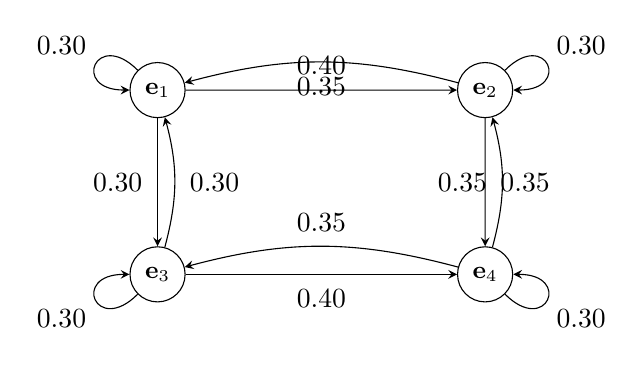
\begin{tikzpicture}[>=stealth, node distance=2.6cm,scale=1.3]
  \tikzset{state/.style={circle, draw, minimum size=7mm, inner sep=0pt, font=\small}}

  \node[state] (e1) at (0,1.8) {\(\e_1\)};
  \node[state] (e2) at (3.2,1.8) {\(\e_2\)};
  \node[state] (e3) at (0,0)   {\(\e_3\)};
  \node[state] (e4) at (3.2,0) {\(\e_4\)};

  %--- neighbor edges (both directions) ---
  % e1 <-> e2
  \draw[->] (e1) -- node[above, yshift=2pt] {\(0.40\)} (e2);
  \draw[->] (e2) to[bend right=15] node[below, yshift=-2pt] {\(0.35\)} (e1);

  % e1 <-> e3
  \draw[->] (e1) -- node[left, xshift=-2pt] {\(0.30\)} (e3);
  \draw[->] (e3) to[bend right=15] node[right, xshift=2pt] {\(0.30\)} (e1);

  % e2 <-> e4
  \draw[->] (e2) -- node[right, xshift=2pt] {\(0.35\)} (e4);
  \draw[->] (e4) to[bend right=15] node[left, xshift=-2pt] {\(0.35\)} (e2);

  % e3 <-> e4
  \draw[->] (e3) -- node[below, yshift=-2pt] {\(0.40\)} (e4);
  \draw[->] (e4) to[bend right=15] node[above, yshift=2pt] {\(0.35\)} (e3);

  %--- self-loops at each state ---
  \draw[->] (e1) edge[out=135, in=180, looseness=7] node[above left] {\(0.30\)} (e1);
  \draw[->] (e2) edge[out=45,  in=0,   looseness=7] node[above right]{\(0.30\)} (e2);
  \draw[->] (e3) edge[out=225, in=180, looseness=7] node[below left] {\(0.30\)} (e3);
  \draw[->] (e4) edge[out=-45, in=0,   looseness=7] node[below right]{\(0.30\)} (e4);
\end{tikzpicture}

\end{center}


\end{frame}



\begin{frame}{Markov chains: finite state space.}

%\begin{deff}
A stochastic process \( (X_0, X_1, \ldots) \) taking values in \( \E \)
is called a \textbf{homogeneous Markov chain} if
$$
\forall n, \forall \e_i, \e_j \in \E:
\quad
\Prob(X_{n+1} = \e_j \mid X_0 = \e_{l_0}, X_1=\e_{l_1},\ldots, X_{n-1}=\e_{l_{n-1}}, X_n = \e_i)=
$$
$$\Prob(X_{n+1} = \e_j \mid X_n = \e_i)
= \Prob(\e_i, \e_j) =\bfP(\e_i,\e_j)\equiv \bfP(i,j).
$$
for every $\e_{l_0}, \e_{l_1},\ldots, \e_{l_{n-1}}, \e_j$ such that
$\Prob( X_0 = \e_{l_0}, X_1=\e_{l_1},\ldots, X_{n-1}=\e_{l_{n-1}}, X_n = \e_i)>0$.
%\end{deff}



\end{frame}


\begin{frame}{Transition matrix and initial distribution.}

\[
\bfP = (\bfP(\e_i,\e_j))_{i,j}\equiv \bfP(i,j)_{i,j}
\]
is the transition matrix of the Markov chain.
If
\[
\forall i,j \quad \bfP(i,j) \ge 0,
\quad
\forall i \quad \sum_j \bfP(i,j) = 1,
\]

then to fully describe the chain we need:
\begin{itemize}
\item the transition matrix \(\bfP\),
\item the initial distribution of \(X_0\).
\end{itemize}

\[
\bfmu^0 \equiv \bfmu = \bfmu^{(0)} =
(\mu(\e_1), \ldots, \mu(\e_m))
= (\Prob(X_0 = \e_1), \ldots, \Prob(X_0 = \e_m)).
\]

Notation:
\[
X \sim (\bfmu, \bfP)
\quad \text{means a Markov chain with transition matrix } \bfP
\text{ and initial distribution } \bfmu.
\]

The distribution after \(k\) steps is
\[
\bfmu^{(n)} =
(\Prob(X_k = \e_1), \Prob(X_k = \e_2), \ldots, \Prob(X_k= \e_m)).
\]

\end{frame}


\begin{frame}{Two viewpoints on a Markov chain.}

\[
\Prob(\e_i,\e_j)=\bfP(\e_i,\e_j)\equiv \bfP(i,j).
\]

\begin{columns}[T,onlytextwidth]
\column{0.55\textwidth}
\textbf{(1) As a directed graph.}

\medskip
\centering
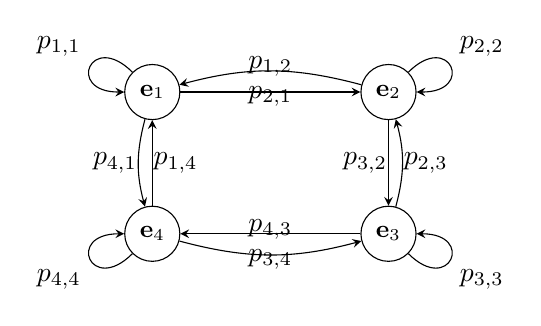
\begin{tikzpicture}[>=stealth, node distance=2.6cm]
  \tikzset{state/.style={circle, draw, minimum size=7mm, inner sep=0pt, font=\small}}

  \node[state] (e1) at (0,1.8) {\(\e_1\)};
  \node[state] (e2) at (3.0,1.8) {\(\e_2\)};
  \node[state] (e3) at (3.0,0)   {\(\e_3\)};
  \node[state] (e4) at (0,0)     {\(\e_4\)};

  % edges between neighbours
  \draw[->] (e1) -- node[above, yshift=2pt] {\(p_{1,2}\)} (e2);
  \draw[->] (e2) -- node[right, xshift=2pt] {\(p_{2,3}\)} (e3);
  \draw[->] (e3) -- node[below, yshift=-2pt]{\(p_{3,4}\)} (e4);
  \draw[->] (e4) -- node[left,  xshift=-2pt]{\(p_{4,1}\)} (e1);

  % the opposite directions, if you want a bidirectional neighbourhood
  \draw[->] (e2) to[bend right=15] node[below, yshift=-2pt]{\(p_{2,1}\)} (e1);
  \draw[->] (e3) to[bend right=15] node[left,  xshift=-2pt]{\(p_{3,2}\)} (e2);
  \draw[->] (e4) to[bend right=15] node[above, yshift=2pt] {\(p_{4,3}\)} (e3);
  \draw[->] (e1) to[bend right=15] node[right, xshift=2pt] {\(p_{1,4}\)} (e4);

  % self-loops everywhere
  \draw[->] (e1) edge[out=135, in=180, looseness=7] node[above left] {\(p_{1,1}\)} (e1);
  \draw[->] (e2) edge[out=45,  in=0,   looseness=7] node[above right]{\(p_{2,2}\)} (e2);
  \draw[->] (e3) edge[out=-45, in=0,   looseness=7] node[below right]{\(p_{3,3}\)} (e3);
  \draw[->] (e4) edge[out=225, in=180, looseness=7] node[below left] {\(p_{4,4}\)} (e4);
\end{tikzpicture}

\column{0.45\textwidth}
\textbf{(2) ``In time''.}

\medskip
% Right column: ``In time''
\centering
% \begin{tikzpicture}[>=stealth, level distance=10mm, sibling distance=16mm]
%   \tikzset{every node/.style={font=\small}}
%
%   % root and first level -- name each child explicitly
%   \node (root) {$X_0=\e_1$}
%     child { node (x1e1) {$X_1=\e_1$} edge from parent node[left]  {$p_{1,1}$} }
%     child { node (x1e2) {$X_1=\e_2$} edge from parent node[left]  {$p_{1,2}$} }
%     child { node (x1e3) {$X_1=\e_3$} edge from parent node[right] {$p_{1,3}$} }
%     child { node (x1e4) {$X_1=\e_4$} edge from parent node[right] {$p_{1,4}$} };
%
%   % second level grown from the named node x1e2
% %   \begin{scope}[grow'=down, level distance=10mm, sibling distance=14mm]
% %     \path (x1e2)
% %       child { node {$X_2=\e_1$} edge from parent node[left]  {$\bfP(2,1)$} }
% %       child { node {$X_2=\e_2$} edge from parent node[right] {$\bfP(2,2)$} };
% %   \end{scope}
% \end{tikzpicture}
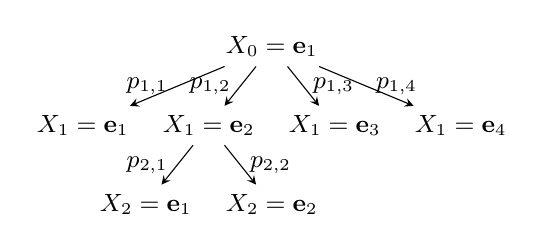
\begin{tikzpicture}[>=stealth, level distance=10mm, sibling distance=16mm]
  \tikzset{every node/.style={font=\small}, edge from parent/.style={->,draw}}

  \node (root) {$X_0=\e_1$}
    child { node {$X_1=\e_1$} edge from parent node[left]  {$p_{1,1}$} }
    child {%
      node (x1e2) {$X_1=\e_2$}
        % grandchildren of X1 = e2
        child { node {$X_2=\e_1$} edge from parent node[left]  {$p_{2,1}$} }
        child { node {$X_2=\e_2$} edge from parent node[right] {$p_{2,2}$} }
      edge from parent node[left] {$p_{1,2}$}
    }
    child { node {$X_1=\e_3$} edge from parent node[right] {$p_{1,3}$} }
    child { node {$X_1=\e_4$} edge from parent node[right] {$p_{1,4}$} };
\end{tikzpicture}



\medskip

\[
\bfP=
\begin{array}{c|cccc}
      & \e_1 & \e_2 & \cdots & \e_m\\\hline
\e_1  & \bfP(1,1) & \bfP(1,2) & \cdots & \bfP(1,M)\\
\e_2  & \bfP(2,1) & \bfP(2,2) & \cdots & \bfP(2,M)\\
\vdots& \vdots & \vdots & \ddots & \vdots\\
\e_m  & \bfP(M,1) & \bfP(M,2) & \cdots & \bfP(m,M)
\end{array}
\]
\end{columns}

\end{frame}



\begin{frame}{Lemma: evolution of the distribution.}

\textbf{Lemma.} For a homogeneous Markov chain \(X \sim (\bfmu,\bfP)\) on \(\E\),
the \(n\)-step distribution is
\[
\bfmu^{(k)} \;=\; \bfmu\,\bfP^{\,k}, \qquad k\ge 0.
\]

\textbf{Proof (by induction).}
\begin{itemize}
\item Base case \(k=1\).
For any \(j\),
\[
\mu^{(1)}(\e_j)=\Prob(X_1=\e_j)
=\sum_{i}\Prob(X_0=\e_i)\,\Prob(X_1=\e_j\mid X_0=\e_i)
=\sum_{i}\mu(\e_i)\,\bfP(i,j).
\]
Hence \(\bfmu^{(1)}=\bfmu\,\bfP\).
\pause
\item Induction step.
Assume \(\bfmu^{(k)}=\bfmu\,\bfP^{\,k}\).
Then, for any \(j\),
$$
\mu^{(k+1)}(\e_j)=\sum_{i}\Prob(X_k=\e_i, X_{k+1}=\e_j)
=\sum_{i}\Prob(X_{k+1}=\e_j| X_k=\e_i)\Prob(X_k=\e_j)$$
$$=\sum_{i}\Prob(X_k=\e_i)\,\bfP(i,j)
=\sum_{i}\mu^{(k)}(\e_i)\,\bfP(i,j).$$
In vector form,
\[
\bfmu^{(k+1)}=\bfmu^{(k)}\bfP
=(\bfmu\,\bfP^{\,k})\,\bfP
=\bfmu\,\bfP^{\,k+1}.
\]
\end{itemize}
\hfill\(\square\)

\end{frame}



\begin{frame}{Example: LA weather — model and transition matrix.}

States: \(\E=\{\e_D,\e_S\}\) where \(\e_D=\) ``dry'', \(\e_S=\) ``sunny''.

\medskip
\begin{columns}[T,onlytextwidth]
\column{0.45\textwidth}
\centering
\begin{tikzpicture}[>=stealth, node distance=32mm]
  \tikzset{state/.style={circle, draw, minimum size=7mm, inner sep=0pt}}
  \node[state] (D) {\(\e_D\)};
  \node[state] (S) [right=of D] {\(\e_S\)};

  % transitions
  \draw[->] (D) to[bend left=20]  node[above] {\(\tfrac12\)} (S);
  \draw[->] (S) to[bend left=20]  node[below] {\(\tfrac1{10}\)} (D);
  \draw[->] (D) edge[out=135,in=180,looseness=7] node[left]  {\(\tfrac12\)} (D);
  \draw[->] (S) edge[out=45, in=0,  looseness=7] node[right] {\(\tfrac9{10}\)} (S);
\end{tikzpicture}

\column{0.55\textwidth}
Transition matrix (rows sum to \(1\)):
\[
\bfP=\begin{pmatrix}
\frac12 & \frac12\\[2pt]
\frac1{10} & \frac9{10}
\end{pmatrix},
\qquad
\Prob(\e_i,\e_j)=\bfP(\e_i,\e_j).
\]

Initial distribution (row vector):
\[
\bfmu=(p,\,1-p).
\]
By the lemma, the distribution at time \(k\) is \(\bfmu^{(k)}=\bfmu\,\bfP^{\,k}\).
\end{columns}

\end{frame}

\begin{frame}{Example: LA weather — spectral decomposition.}

We start from
\[
\bfP=
\begin{pmatrix}
\frac12 & \frac12\\[2pt]
\frac1{10} & \frac9{10}
\end{pmatrix}.
\]

We diagonalize \(\bfP\):
\[
\lambda_1=1,\qquad \lambda_2=\tfrac25,
\]
\[
A=\begin{pmatrix}1 & -5\\[2pt]1 & 1\end{pmatrix},
\qquad
A^{-1}=\begin{pmatrix}\tfrac16 & \tfrac56\\[2pt]-\tfrac16 & \tfrac16\end{pmatrix}.
\]

\[
\bfP = A D A^{-1},
\quad
D=\begin{pmatrix}\lambda_1 & 0\\[2pt]0 & \lambda_2\end{pmatrix}.
\]

\end{frame}




\begin{frame}{Example: LA weather — spectral decomposition.}


\[
\bfP^{\,k} = A D^{\,k} A^{-1}
= A
\begin{pmatrix}1 & 0\\[2pt]0 & (\tfrac25)^{k}\end{pmatrix}
A^{-1}.
\]
Compute:
\[
A D^{\,k} A^{-1}
=
\begin{pmatrix}1 & -5\\[2pt]1 & 1\end{pmatrix}
\begin{pmatrix}1 & 0\\[2pt]0 & (\tfrac25)^k\end{pmatrix}
\begin{pmatrix}\tfrac16 & \tfrac56\\[2pt]-\tfrac16 & \tfrac16\end{pmatrix}.
\]

After multiplication,
\[
\bfP^{\,k} =
\begin{pmatrix}
\frac16+\frac56(\tfrac25)^k & \frac56-\frac56(\tfrac25)^k\\[4pt]
\frac16-\frac16(\tfrac25)^k & \frac56+\frac16(\tfrac25)^k
\end{pmatrix}.
\]

\[
\text{If }\bfmu=(p,1-p),\quad
\bfmu\,\bfP^{\,k}=
\Bigl(
\tfrac16+(\tfrac25)^k p,\;
\tfrac56-(\tfrac25)^k p
\Bigr)
\xrightarrow[k\to\infty]{}
\Bigl(\tfrac16,\tfrac56\Bigr).
\]

% \textbf{Hence} the stationary distribution is
% \[
% \bfpi = (\tfrac16,\tfrac56),
% \qquad
% \bfpi\,\bfP=\bfpi,
% \quad
% \sum_i\bfpi(i)=1.
% \]
\end{frame}



\begin{frame}{Example: Ehrenfest model.}

We have \(N\) particles distributed between boxes \(A\) and \(B\).
At each step one particle is chosen uniformly at random and moved to the other box.

\medskip
\textbf{State:} \(X_n = i\) means that box \(A\) contains \(i\) particles
(\(0 \le i \le N\)).

\begin{center}
\begin{tikzpicture}[>=stealth, node distance=1.2cm, font=\small]
  \node (0) at (0,0) {0};
  \node (1) at (1.2,0) {1};
  \node (i) at (2.7,0) {\(i\)};
  \node (ip1) at (4.2,0) {\(i{+}1\)};
  \node (N) at (5.8,0) {\(N\)};

  \draw[->] (1) -- (0) node[midway, above] {\(\tfrac1N\)};
  \draw[->] (i) -- (ip1) node[midway, above] {\(\tfrac{N-i}{N}\)};
  \draw[->] (i) -- (1.2,0) node[pos=0.35, below] {\(\tfrac{i}{N}\)};
\end{tikzpicture}
\end{center}

Transition probabilities:
\[
\Prob(X_{n+1}=i-1 \mid X_n=i)=\frac{i}{N},\qquad
\Prob(X_{n+1}=i+1 \mid X_n=i)=\frac{N-i}{N}.
\]

\[
\bfP =
\begin{pmatrix}
0 & 1 & 0 & \cdots & 0\\[2pt]
\frac1N & 0 & \frac{N-1}{N} & \cdots & 0\\[2pt]
0 & \frac2N & 0 & \cdots & 0\\
\vdots & & \ddots & & \vdots\\
0 & \cdots & 0 & \frac{N}{N} & 0
\end{pmatrix}.
\]
\end{frame}


\begin{frame}{Example: Top-2-random model.}

We consider a permutation Markov chain on \(S_n\), e.g. \(n=3\).
At each step we randomly choose one of the two top elements and move it to the top.

\medskip
For \(n=3\), states can be written as:
\[
\E = \{ (1,2,3), (1,3,2), (2,1,3), (2,3,1), (3,1,2), (3,2,1) \}.
\]

\[
\bfP =
\begin{array}{c|cccccc}
 & (1,2,3) & (2,1,3) & (2,3,1) & \ldots  \\ \hline
(1,2,3) & \tfrac13 & \tfrac13 & \tfrac13 \\
(2,1,3) & \ddots \\
\vdots &
\end{array}
\quad \text{(and similarly for other states)}.
\]

\end{frame}




\begin{frame}{Example: Top-2-random model.}


\medskip
However, the matrix \(\bfP\) is large and cannot be written explicitly for general \(n\).
It is more convenient to describe transitions \emph{locally}:
\[
\Prob(\e_i,\e_j) =
\begin{cases}
\tfrac1n, & \text{if } \e_j \text{ is obtained from } \e_i \text{ by moving one of the top 2 elements to the top},\\[4pt]
0, & \text{otherwise.}
\end{cases}
\]

\begin{center}
\begin{tikzpicture}[>=stealth, node distance=2cm, font=\small]
  \node (e1) at (0,0) {\((1,2,3)\)};
  \node (e2) at (2.5,1) {\((1,3,2)\)};
  \node (e3) at (2.5,-1) {\((2,1,3)\)};
  \draw[->] (e1) to[bend left=10] node[above] {\(\tfrac13\)} (e2);
  \draw[->] (e1) to[bend right=10] node[below] {\(\tfrac13\)} (e3);
  \draw[->] (e1) edge[out=135,in=180,looseness=7] node[left] {\(\tfrac13\)} (e1);
\end{tikzpicture}
\end{center}

\end{frame}


\begin{frame}{How to simulate a Markov chain \(X\sim(\bfmu,\bfP)\): sampling \(X_0\).}

Example initial distribution:
\[
\bfmu=(\tfrac14,\ \tfrac12,\ 0,\ \tfrac14)
\quad\text{on}\quad
\E=\{\e_1,\e_2,\e_3,\e_4\}.
\]

Draw \(U_0\sim \mathsf{U}(0,1)\) and set
\[
X_0=\begin{cases}
\e_1, & U_0\in[0,\tfrac14),\\
\e_2, & U_0\in[\tfrac14,\tfrac34),\\
\e_3, & \text{never (mass \(0\))},\\
\e_4, & U_0\in[\tfrac34,1].
\end{cases}
\]

\medskip
\centering
\begin{tikzpicture}[x=10cm,y=1cm,font=\small,>=stealth]
  % baseline
  \draw (0,0) -- (1,0);
  % ticks
  \foreach \x/\lab in {0/0,0.25/\tfrac14,0.75/\tfrac34,1/1} {
    \draw (\x,0.08) -- (\x,-0.08) node[below=3pt] {\(\lab\)};
  }
  % segments with labels
  \draw[thick] (0,0) -- (0.25,0) node[midway,above=4pt] {\(\e_1\)};
  \draw[thick] (0.25,0) -- (0.75,0) node[midway,above=4pt] {\(\e_2\)};
  % e3 has zero length; show a small marker at 0.75 (optional)
  \fill (0.75,0) circle (0.8pt) node[above=4pt] {\(\e_3\)};
  \draw[thick] (0.75,0) -- (1,0) node[midway,above=4pt] {\(\e_4\)};
\end{tikzpicture}

\end{frame}
\begin{frame}{Initialization and update functions.}

Let \(U_0,U_1,U_2,\ldots\) be i.i.d.\ \(\mathsf{U}(0,1)\).

\textbf{Initialization function} \(\psi:[0,1]\to\E\) such that for all \(\e_j\in\E\),
\[
\int_0^1 \mathbf{1}\{\psi(x)=\e_j\}\,dx \;=\; \bfmu(\e_j).
\]
A canonical choice using cumulative sums:
\[
\psi(x)=
\begin{cases}
\e_1, & x\in\big[0,\ \bfmu(\e_1)\big),\\
\e_j, & x\in\Big[\sum_{s=1}^{j-1}\bfmu(\e_s),\ \sum_{s=1}^{j}\bfmu(\e_s)\Big),\ \ j=2,\ldots,M.
\end{cases}
\]
Set \(X_0=\psi(U_0)\).

\end{frame}




\begin{frame}{Initialization and update functions.}

\medskip
\textbf{Update function} \(\varphi:\E\times[0,1]\to\E\) encodes one Markov step of \(\bfP\):
for each fixed \(\e_i\) and all \(\e_j\),
\[
\int_0^1 \mathbf{1}\{\varphi(\e_i,x)=\e_j\}\,dx \;=\; \bfP(\e_i,\e_j).
\]
A convenient definition via row–wise cumulative sums of \(\bfP\):
\[
\varphi(\e_i,x)=
\begin{cases}
\e_1, & x\in\big[0,\ \bfP(\e_i,\e_1)\big),\\
\e_j, & x\in\Big[\sum_{s=1}^{j-1}\bfP(\e_i,\e_s),\ \sum_{s=1}^{j}\bfP(\e_i,\e_s)\Big),\ \ j=2,\ldots,m.
\end{cases}
\]
\pause
\medskip
\textbf{Simulation:} given \(X_0=\psi(U_0)\), generate \(X_{n+1}=\varphi(X_n,U_{n+1})\) for \(n\ge 0\).

\end{frame}

\begin{frame}{Irreducible Markov chains.}

\textbf{Def.}
A homogeneous Markov chain \(X\sim(\bfmu,\bfP)\) with state space \(\E=\{\e_1,\ldots,\e_m\}\)
is called \textbf{irreducible} if for all states \(\e_i,\e_j\in\E\)
there exists an integer \(N_{ij}\ge1\) such that
\[
\Prob(X_{N_{ij}}=\e_j\mid X_0=\e_i)>0
\quad\Longleftrightarrow\quad
\bfP^{N_{ij}}(\e_i,\e_j)>0.
\]


That is, each state can be reached from any other with positive probability
in a finite number of steps.

\medskip
For irreducible \(\bfP\) the corresponding graph is   connected.
\end{frame}
\begin{frame}{Period and aperiodicity.}

\textbf{Def.}
The \textbf{period} of a state \(\e_i\) is defined as
\[
d(\e_i) = \gcd\{\, n\ge1 : \bfP^{n}(\e_i,\e_i)>0\,\}.
\]


A state \(\e_i\) is \textbf{aperiodic} if \(d(\e_i)=1\).

\pause
\medskip
\textbf{Def.}
A chain \(X\sim(\bfmu,\bfP)\) is \textbf{aperiodic} if all its states are aperiodic,
that is,
\[
d(\e_i)=1\quad\text{for all } \e_i\in\E.
\]


\end{frame}

\begin{frame}{Characterization theorem and Bremaud's lemma.}

\textbf{Theorem.}
If \(X\sim(\bfmu,\bfP)\) is irreducible,
then there exists \(N_0<\infty\) such that
\[
\forall\, (\e_i \in\E),\quad \forall\, (n\geq N)\qquad  \bfP^{n}(\e_i,\e_i)>0.
\]

\medskip
\textbf{Idea of proof.}

By a lemma due to Bremaud:
if a set \(A\subset\mathbb{N}\) satisfies
\begin{enumerate}
\item \(\gcd(A)=1\);
\item \(a,a'\in A \implies a+a'\in A\);
\end{enumerate}
then there exists \(N<\infty\) such that all \(n>N\) belong to \(A\).

\end{frame}



\begin{frame}{Characterization theorem and Bremaud's lemma.}


For each state \(\e_i\) define
\[
A_i = \{\,n\ge1:\ \bfP^{n}(\e_i,\e_i)>0\,\},\qquad
\]
State $\e_i$ is aperiodic, i.e., $d(\e_i)=\gcd(A_i)=1.$
Note:
$$\bfP^{a+a'}(\e_i,\e_i)=\Prob(X_{a+a'}=\e_i|X_0=\e_i) \geq
\Prob(X_{a}=\e_i|X_0=\e_i)\Prob(X_{a'}=\e_i|X_0=\e_i)$$
i.e. $a,a'\in A_i \implies a+a'\in A$.
\begin{center}
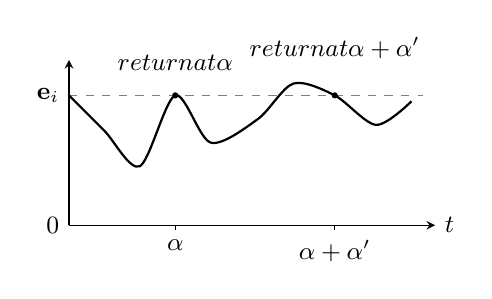
\begin{tikzpicture}[>=stealth, scale=0.75, font=\small]
  % axes
  \draw[->] (0,0) -- (6.2,0) node[right] {\(t\)};
  \draw[->] (0,0) -- (0,2.8);

  % labels
  \node[left] at (0,2.2) {\(\e_i\)};
  \node[left] at (0,0) {0};

  % ticks
  \draw (1.8,0) -- (1.8,-0.08) node[below] {\(\alpha\)};
  \draw (4.5,0) -- (4.5,-0.08) node[below] {\(\alpha+\alpha'\)};

  % horizontal line for e_i level
  \draw[dashed, gray] (0,2.2) -- (6.0,2.2);

  % trajectory: starts and returns to e_i at alpha and alpha+alpha'
  \draw[smooth,thick]
    plot coordinates {
      (0,2.2)
      (0.6,1.6)
      (1.2,1.0)
      (1.8,2.2)
      (2.4,1.4)
      (3.2,1.8)
      (3.8,2.4)
      (4.5,2.2)
      (5.2,1.7)
      (5.8,2.1)
    };

  % markers for returns
  \filldraw (1.8,2.2) circle (1.2pt);
  \filldraw (4.5,2.2) circle (1.2pt);

  % annotations
  \node at (1.8,2.45) [above] {\(\text{return at }\alpha\)};
  \node at (4.5,2.65) [above] {\(\text{return at }\alpha+\alpha'\)};
\end{tikzpicture}
\end{center}
\pause
\medskip
Taking $N=\max_i N_i$ we have that
$$\forall\, (\e_i \in\E),\quad \forall\, (n\geq N)\qquad  \bfP^{n}(\e_i,\e_i)>0.$$

\end{frame}


 \begin{frame}{Irreducible + aperiodic $\Rightarrow$ uniform positivity.}

\textbf{Theorem.}
If $X\sim(\bfmu,\bfP)$ is irreducible and aperiodic,
then $\exists\,N_0<\infty$ such that
\[
\forall\,\e_i,\e_j\in\E,\quad \bfP^{N_0}(\e_i,\e_j)>0.
\]

\textbf{Proof.}
From the previous theorem (aperiodic case),
\[
\exists\,N<\infty\ \text{such that}\
\forall\,i,\quad \bfP^{N}(\e_i,\e_i)>0.
\]
\pause
By irreducibility, for each pair $(i,j)$
there exists $r_{ij}\ge1$ with
\(\bfP^{r_{ij}}(\e_i,\e_j)>0\).
Then for all \(n\ge N+r_{ij}\),
\[
\bfP^{n}(\e_i,\e_j)
\;\ge\;
\bfP^{r_{ij}}(\e_i,\e_j)\,\bfP^{N}(\e_j,\e_j)
>0.
\]
\pause
Since the state space is finite, setting
\[
N_0 = N + \max_{i,j} r_{ij}
\]
gives $\bfP^{N_0}(\e_i,\e_j)>0$ for all $(i,j)$.
\hfill$\square$

\end{frame}


\begin{frame}{Stationary distribution.}

\textbf{Def.}
For a homogeneous Markov chain \(X\sim(\bfmu,\bfP)\) on \(\E=\{\e_1,\ldots,\e_m\}\),
a probability vector
\[
\bfpi = \big(\pi(\e_1),\ldots,\pi(\e_m)\big)
\]
is called a \textbf{stationary distribution} of \(X\) if
\[
\bfpi\,\bfP = \bfpi,
\qquad
\pi(\e_i)>0,
\qquad
\sum_{i=1}^{m}\pi(\e_i)=1.
\]

\end{frame}

\begin{frame}{Example: stationary distribution – LA weather model.}

Recall that
\[
\bfP=
\begin{pmatrix}
\frac12 & \frac12\\[2pt]
\frac1{10} & \frac9{10}
\end{pmatrix}.
\]

Previously we found that if \(\bfmu=(p,1-p)\), then
\[
\bfmu\,\bfP^{\,k}=
\Bigl(
\tfrac16+(\tfrac25)^k p,\;
\tfrac56-(\tfrac25)^k p
\Bigr)
\xrightarrow[k\to\infty]{}
\bfpi=\Bigl(\tfrac16,\tfrac56\Bigr).
\]

\medskip
\textbf{Observation.}
The limit \(\bfpi\) satisfies the stationarity condition:
\[
\bfpi\,\bfP = \bfpi,
\qquad
\text{i.e.}\quad
\begin{pmatrix}
\tfrac16 & \tfrac56
\end{pmatrix}
\begin{pmatrix}
\frac12 & \frac12\\[2pt]
\frac1{10} & \frac9{10}
\end{pmatrix}
=
\begin{pmatrix}
\tfrac16 & \tfrac56
\end{pmatrix}.
\]

Thus, \(\bfpi\) is the \textbf{stationary distribution} of the LA weather chain.

\end{frame}

\begin{frame}{Stationarity is preserved over time.}

\textbf{Lemma.}
If the initial distribution equals a stationary distribution, i.e.\ $\bfmu=\bfpi$ and $\bfpi\,\bfP=\bfpi$,
then for every $k\ge 0$ the law of $X_k$ is $\bfpi$.

\bigskip
\textbf{Proof.}
From the evolution formula $\bfmu^{(k)}=\bfmu\,\bfP^{\,k}$, putting $\bfmu=\bfpi$ gives
\[
\bfmu^{(k)}=\bfpi\,\bfP^{\,k}.
\]
Since $\bfpi\,\bfP=\bfpi$, multiplying by $\bfP$ repeatedly yields
$\bfpi\,\bfP^{\,k}=\bfpi$ for all $k\ge 0$.
Hence $\bfmu^{(k)}=\bfpi$ for every $k$. \hfill$\square$

\end{frame}


\begin{frame}{Return and hitting times.}

\textbf{Def.}
For a Markov chain \(X\sim(\bfmu,\bfP)\), define
\[
T_{ij} = \min\{\,n\ge1 : X_n = \e_j,\ X_0 = \e_i\,\}.
\]

\textbf{Lemma.}
If \(X\) is irreducible and aperiodic, then
\[
\forall\,i,j,\quad \Prob(T_{ij}<\infty)=1.
\]

\textbf{Proof.}
From the previous theorem, there exists \(N_0<\infty\) such that
\[
\forall\,i,j,\quad \bfP^{N_0}(\e_i,\e_j)>0.
\]
Let
\[
\lambda = \min_{i,j} \bfP^{N_0}(\e_i,\e_j) > 0.
\]

Then, starting from \(\e_i\),
\[
\Prob(T_{ij}>N_0) \leq  \Prob(X_{N_0}\neq \e_j \mid X_0=\e_i) = 1 - \Prob(X_{N_0}=\e_j \mid X_0=\e_i)
\le 1 - \lambda.
\]


\end{frame}




\begin{frame}{Return and hitting times.}
For \(2N_0\),
$$
\Prob(T_{ij}>2N_0)=\Prob(T_{ij}>N_0)\Prob(T_{ij}>2N_0|T_{ij}>N_0)
$$
$$
\leq \Prob(T_{ij}>N_0)\Prob(X_{2N_0}\neq\e_j\mid T_{ij}>N_0)
$$
$$\leq (1-\lambda)(1-\lambda)=(1-\lambda)^2
$$

\pause

By induction,
\[
\Prob(T_{ij}>kN_0) \le (1-\lambda)^k,
\qquad k=1,2,\ldots
\]

Hence
\[
\Prob(T_{ij}<\infty)
= 1 - \lim_{k\to\infty}\Prob(T_{ij}>kN_0)
= 1.
\]
\hfill$\square$

\end{frame}

\begin{frame}{Expected hitting time is finite.}

\textbf{Lemma.}
If $X\sim(\bfmu,\bfP)$ is irreducible and aperiodic, then for all $i,j$
the hitting time $T_{ij}=\min\{n\ge1: X_n=\e_j,\ X_0=\e_i\}$ satisfies
\[
\Exp[T_{ij}]<\infty .
\]

\textbf{Proof.}
By the previous theorem, $\exists\,N_0<\infty$ with
$\bfP^{N_0}(\e_a,\e_b)>0$ for all $a,b$; set
\[
\lambda \;=\; \min_{a,b}\,\bfP^{N_0}(\e_a,\e_b)\;>\;0.
\]
Then for $k=1,2,\dots$,
\[
\Prob(T_{ij}>kN_0)\;\le\; (1-\lambda)^k
\quad\Rightarrow\quad
\Prob(T_{ij}>n)\;\le\;(1-\lambda)^{\lfloor n/N_0\rfloor}.
\]
\pause
Using the tail-sum formula and grouping $n$ into blocks of length $N_0$,
\[
\Exp[T_{ij}]=\sum_{n\ge0}\Prob(T_{ij}>n)
\;\le\;\sum_{h=0}^{\infty}\;\sum_{n=hN_0}^{(h+1)N_0-1}\Prob(T_{ij}>n)
\;\le\;\sum_{h=0}^{\infty} N_0\,(1-\lambda)^h
\;=\;\frac{N_0}{\lambda}\;<\;\infty.
\]
\hfill$\square$

\end{frame}

\begin{frame}{Existence of a stationary distribution (construction).}

\textbf{Theorem.}
If $X\sim(\bfmu,\bfP)$ is irreducible and aperiodic on $\E=\{\e_1,\dots,\e_M\}$,
then there exists a stationary distribution $\bfpi$.
\medskip\par
\pause
\textbf{Construction.}
Start from $\e_1$ and define the return time
\[
T_{11}=\min\{n\ge1:X_n=\e_1\mid X_0=\e_1\}.
\]
For $i=1,\dots,M$ set
\[
s_i \;=\; \Exp_{\,\e_1}\!\Bigg[\sum_{n=0}^{T_{11}-1}\mathbf{1}\{X_n=\e_i\}\Bigg]
\quad\text{(expected \# of visits to $\e_i$ before the return to $\e_1$).}
\]
\pause
Define
\[
\bfpi \;=\; \frac1{\Exp_{\,\e_1}[T_{11}]}\,\big(s_1,\dots,s_m\big).
\]
 We have already shown that  $\Exp_{\e_1}[T_{11}]<\infty$.  ,

\end{frame}

\begin{frame}{Normalization: finiteness and $\sum_i s_i=\Exp_{\e_1}[T_{11}]$.}


\textbf{Sum of $s_i$.}
For every trajectory,
\(
\sum_{i=1}^M \sum_{n=0}^{T_{11}-1}\mathbf{1}\{X_n=\e_i\}=T_{11}
\)
(because at each $n<T_{11}$ the chain is in exactly one state).
Taking expectation,
$$
\sum_{i=1}^M s_i
=\sum_{i=1}^M  \Exp_{\,\e_1}\!\Bigg[\sum_{n=0}^{T_{11}-1}\mathbf{1}\{X_n=\e_i\}\Bigg]
$$
$$
= \Exp_{\,\e_1}\sum_{i=1}^M \!\Bigg[\sum_{n=0}^{T_{11}-1}\mathbf{1}\{X_n=\e_i\}\Bigg] =\Exp_{\e_1}[T_{11}].
$$

Hence $  \bfpi \;=\; \frac1{\Exp_{\,\e_1}[T_{11}]}\,\big(s_1,\dots,s_M\big)  $ is a probability vector with strictly positive components.
\end{frame}

\begin{frame}{Stationarity: $\sum_i s_i\,\bfP(\e_i,\e_j)=s_j$.}

Fix $j$. Write
\[
s_j=\Exp_{\e_1}\!\Bigg[\sum_{n=0}^{T_{11}-1}\mathbf{1}\{X_n=\e_j\}\Bigg]
=\sum_{n=0}^{\infty}\Prob_{\e_1}\big(X_n=\e_j,\;T_{11}>n\big).
\tag{1}
\]
For $n\ge0$ use the Markov property on the event $\{T_{11}>n\}$ (so $X_n\neq \e_1$):
\[
\Prob_{\e_1}(X_{n+1}=\e_j,\,T_{11}>n+1)
=\sum_{i=1}^M \Prob_{\e_1}(X_n=\e_i,\,T_{11}>n)\,\bfP(\e_i,\e_j).
\tag{2}
\]
Summing \((2)\) over $n\ge0$ and comparing with \((1)\):
\[
\sum_{i=1}^M \bfP(\e_i,\e_j)\,\Bigg[\sum_{n=0}^{\infty}
\Prob_{\e_1}(X_n=\e_i,\,T_{11}>n)\Bigg]
=\sum_{n=0}^{\infty}\Prob_{\e_1}(X_{n+1}=\e_j,\,T_{11}>n+1).
\]
The bracket equals $s_i$ by definition; the RHS equals $s_j$
(a mere reindexing $n\mapsto n-1$ in \((1)\)).
Therefore \(\sum_i s_i\,\bfP(\e_i,\e_j)=s_j\) for all $j$, i.e.
$$
\big(s_1,\dots,s_m\big)\,\bfP=\big(s_1,\dots,s_m\big).
\qquad \textrm{Dividing\ by } \Exp_{\e_1}[T_{11}]
\ \textrm{yields}\ \bfpi\,\bfP=\bfpi $$

\end{frame}

% --- 1. Cel + metryka TV ---
\begin{frame}{Convergence to stationarity in total variation.}
\textbf{Total variation norm.}
For probability vectors \(\mu,\nu\) on \(\E\),
\[
d_{\rm TV}(\mu,\nu)\;=\;\tfrac12\sum_{\e\in\E}|\mu(\e)-\nu(\e)|\;\in[0,1].
\]

\textbf{Goal.} For a finite, irreducible and aperiodic chain \(X\sim(\bfmu,\bfP)\) on
\(\E=\{\e_1,\dots,\e_M\}\) with stationary law \(\bfpi\), show
\[
d_{\rm TV}\!\big(\bfmu\,\bfP^{\,k},\bfpi\big)\xrightarrow[k\to\infty]{}0.
\]


\pause
\textbf{Idea (coupling). }We construct two chains driven by a common source of randomness and show that they eventually \emph{merge}.
Then, the difference between their distributions at time
$k$ bounded by the probability that they have not yet merged by time
$k$
\end{frame}


% --- 2. Konstrukcja coupling'u ---
\begin{frame}{Coupling via update/initialization maps.}
\textbf{Coupling $(X_k,Y_k)$} of Markov chains with t.m. $\bfP$. Marginally $(X_k)\sim \bfP$ and $(Y_k)\sim\bfP$.
\medskip\par
Let \(U_0,U_1,\ldots \stackrel{\text{i.i.d.}}{\sim}\mathrm{Unif}(0,1)\).
Use an initialization map \(\psi_\rho:[0,1]\to\E\) for a law \(\rho\),
and an update map \(\varphi:\E\times[0,1]\to\E\) such that
\[
X_0=\psi_{\bfmu}(U_0),\qquad X_{n+1}=\varphi(X_n,U_{n+1})
\]
generates \(X\sim(\bfmu,\bfP)\).
Independently set
\[
X_0'=\psi_{\bfpi}(U_0'),\qquad X_{n+1}'=\varphi(X_n',U_{n+1}'),
\]
with \(U_0',U_1',\ldots\) i.i.d.\ \(\mathrm{Unif}(0,1)\), independent of \((U_n)\).
Then \(X_n'\sim\bfpi\) for all \(n\) (by \(\bfpi\,\bfP=\bfpi\)).

\end{frame}



\begin{frame}{Coupling via update/initialization maps.}


\textbf{Coupling time.}
\[
T=\min\{n\ge0:\;X_n=X_n'\}.
\]

\begin{center}
\includegraphics[width=0.6\linewidth]{pics/coupling_indep.png}
\end{center}

We will show a geometric tail for \(T\) and conclude \(d_{\rm TV}(\bfmu\bfP^{\,k},\bfpi)\le \Prob(T>k)\to0\).
\end{frame}



% --- 3. Ujednolicone minorization + ogon T ---
\begin{frame}{Uniform positivity $\Rightarrow$ geometric tail of the coupling time.}

\textbf{Lemma (minorization).}
For finite irreducible aperiodic chains there exist \(N_0\in\mathbb{N}\) and \(\lambda>0\) such that
\[
\min_{i,j}\,\bfP^{N_0}(\e_i,\e_j)\;\ge\;\lambda.
\]

\textbf{Consequence.}
Independently of \(X_0,X_0'\),
\[
\Prob\big(X_{N_0}=\e_1\big)\;\ge\;\lambda,\qquad
\Prob\big(X_{N_0}'=\e_1\big)\;\ge\;\lambda,
\]
hence
\[
\Prob(T\le N_0)\;\ge\;\Prob\big(X_{N_0}=X_{N_0}'=\e_1\big)\;\ge\;\lambda^2.
\]
By restarting the argument after each block of length \(N_0\),
\[
\Prob(T>kN_0)\;\le\;(1-\lambda^2)^{k},\qquad k=1,2,\ldots
\]

\end{frame}


 \begin{frame}{Coupling via a third chain \(X''\)}
\small
\textbf{Setup.} Let the state space be \(E=\{\e_1,\ldots,\e_m\}\).
Fix an \emph{update map} \(\varphi:E\times[0,1]\to E\) and \emph{initializers} \(\psi_{\nu}:[0,1]\to E\) so that:
\[
X_0=\psi_{\bfmu}(U_0),\qquad X_n=\varphi(X_{n-1},U_n),\quad n\ge1,
\]
\[
X'_0=\psi_{\bfpi}(U'_0),\qquad X'_n=\varphi(X'_{n-1},U_n),\quad n\ge1,
\]
where \((U_0,U_1,\ldots)\) and \(U'_0\) are i.i.d.\ \(\mathrm{Unif}(0,1)\), independent, and \(\bfpi\bfP=\bfpi\).
Then \(X\sim(\bfmu,\bfP)\) and \(X'\sim(\bfpi,\bfP)\) with \(X'_n\sim\bfpi\) for every \(n\).

\medskip
\textbf{Meeting time.} Define the coupling (meeting) time
\[
T:=\min\{n\ge0:\;X_n=X'_n\}.
\]

\end{frame}



 \begin{frame}{Coupling via a third chain \(X''\)}

\[
T:=\min\{n\ge0:\;X_n=X'_n\}.
\]

\textbf{Third chain.} Using the same driving sequence \((U_1,U_2,\ldots)\), define
\[
X''_n \;=\; \begin{cases}
X_n, & n<T,\\[2pt]
X'_n, & n\ge T.
\end{cases}
\]
\begin{center}
\includegraphics[width=0.6\linewidth]{pics/coupling_indep3.png}
\end{center}

\end{frame}



 \begin{frame}{Coupling via a third chain \(X''\)}

\begin{center}
\includegraphics[width=0.4\linewidth]{pics/coupling_indep3.png}
\end{center}
\emph{Claim:} \((X''_n)_{n\ge0}\) is a Markov chain with kernel \(\bfP\) and initial law \(\bfmu\).
\begin{itemize}\itemsep2pt
\item For \(n<T\), \(X''_n=X_n\) so the one-step update is \(X''_{n+1}=\varphi(X_n,U_{n+1})\), i.e.\ kernel \(\bfP\).
\item At time \(T\), \(X''_T=X'_T\). Thereafter, \(X''_{T+k}=\varphi(X''_{T+k-1},U_{T+k})\), again with kernel \(\bfP\).
\item Since \(X''_0=X_0=\psi_{\bfmu}(U_0)\), we have \(\mathcal{L}(X''_0)=\bfmu\).
\end{itemize}
Hence \(X''\sim(\bfmu,\bfP)\). In particular, for each \(n\),
\[
\mathcal{L}(X''_n)=\bfmu\bfP^{\,n}=: \bfmu^{(n)}, \qquad \mathcal{L}(X'_n)=\bfpi.
\]
\end{frame}


\begin{frame}{Bounding \(d_{\rm TV}\) and convergence to \(\bfpi\)}
\small
Fix \(n\ge0\). Since \(X''_n\sim\bfmu^{(n)}\) and \(X'_n\sim\bfpi\),
\[
d_{\rm TV}\!\left(\bfmu^{(n)},\bfpi\right)
=\max_{A\subseteq E}\big|\Prob(X''_n\in A)-\Prob(X'_n\in A)\big|.
\]
For any \(A\subseteq E\),
\[
\begin{aligned}
\big|\Prob(X''_n\in A)-\Prob(X'_n\in A)\big|
&=\big|\Prob(X''_n\in A,\,X'_n\notin A)-\Prob(X'_n\in A,\,X''_n\notin A)\big|\\
&\le \Prob\big(X''_n\neq X'_n\big)
= \Prob(T>n).
\end{aligned}
\]
Therefore
\[
d_{\rm TV}\!\left(\bfmu^{(n)},\bfpi\right)\;\le\;\Prob(T>n).
\]

\medskip
\textbf{Tail of \(T\).} (From irreducibility + aperiodicity.)
There exist \(N_0\in\mathbb{N}\) and \(\lambda>0\) such that
\[
\min_{i,j}\, \bfP^{N_0}(\e_i,\e_j)\;\ge\;\lambda
\quad\Longrightarrow\quad
\Prob(T\le N_0)\;\ge\;\lambda^2,
\]
hence by the strong Markov property,
\[
\Prob(T>kN_0)\;\le\;(1-\lambda^2)^k\;\xrightarrow[k\to\infty]{}\;0.
\]

\medskip
\textbf{Conclusion.} $\qquad \displaystyle
\lim_{n\to\infty} d_{\rm TV}\!\left(\bfmu^{(k)},\bfpi\right)=0,
\qquad\text{i.e.}\quad \bfmu^{(k)}\to\bfpi.
$
\end{frame}

\begin{frame}[t]{Uniqueness of the stationary distribution}

\textbf{Lemma.}
For a finite, irreducible and aperiodic Markov chain with transition matrix \(\bfP\),
there is at most one stationary distribution \(\bfpi\)
(i.e.\ a probability row vector satisfying \(\bfpi=\bfpi\bfP\)).

\medskip
\textbf{Proof.}
Suppose \(\bfpi\) and \(\bfpi'\) are both stationary:
\(\bfpi=\bfpi\bfP\) and \(\bfpi'=\bfpi'\bfP\).
By the convergence theorem proved earlier, for any initial law \(\bfmu\),
\[
\bfmu\,\bfP^{\,n}\xrightarrow[n\to\infty]{d_{\rm TV}} \bfpi .
\]
Take \(\bfmu=\bfpi'\).
Since \(\bfpi'\) is stationary, \(\bfpi'\bfP^{\,n}=\bfpi'\) for all \(n\),
so the same limit must equal \(\bfpi'\):
\[
\bfpi'=\lim_{n\to\infty}\bfpi'\bfP^{\,n}
=\lim_{n\to\infty}\bfmu\,\bfP^{\,n}
=\bfpi.
\]
Therefore \(\bfpi'=\bfpi\),
hence the stationary distribution is unique.
\hfill$\square$

\end{frame}


\end{document}

